\section{Алгоритм деформации }

\subsection{Описание алгоритма}
Базовым средством изменения геометрии фигуры является инструмент ``деформация''.
С помощью этого инструмента пользователь может скорректировать геометрию
загруженного объекта.

Использование инструмента происходит по следующей схеме

\begin{enumerate}
    \item Пользователь активирует инструмент в меню инструментов
    \item После наведения мышки на модель, появляется сфера, демонстрирующая
    изменения, которые произойдут с геометрией после применения инструмента на
    этом участке модели.
    \item После одиночного щелчка мыши вершины геометрии, которые попали во
    внутрь сферы, будут спроецированы на ее переднюю поверхность
\end{enumerate}

Инструмент реализован в рамках поведенческого шаблона Strategy. Интересной
особенностью этого инструмента является то, что, ввиду необходимости добавлять
схематичную сферу на сцену для демонстрации последствий деформации, инструмент
вынужден вмешиваться в процесс отображения сцены, при этом не добавляя
дополнительных логических связей между собой и другими модулями приложения. Это
было достигнуто следующим образом.

При создании инструмента (а инструменты создаются непосредственно перед моментом
своей установки) в личном пространстве имен сохраняется функция,
выполняющую отображение сцены.

\begin{lstlisting}
function ModifyingStrategy(mobject) {
    this.managedObject = mobject;
    this.formerRender = mobject.render;
}
\end{lstlisting}

Теперь, в связки с возможностью передавать функциям любой объект,
выступающий в роли ``this'', у нас есть возможность полностью подменить функцию
отображения сцены

\begin{lstlisting}
ModifyingStrategy.prototype.setUp = function() {
    var gthis = this;
    this.managedObject.render = function() {
        // Adding sphere is needed
        ....
        // Calling original rendering method
        gthis.formerRender.call(this);
    }
}
\end{lstlisting}

В класс-ориентированных языках программирования подобный прием мог быть
реализован с помощью наследования и переопределения
виртуальных функций, с последующим вызовом супер-реализации этой функции.

Для того, чтобы задать правильные координаты сферы в сцене, необходимо решить
задачу нахождения координат точки в трехмерном пространстве сцены, на которую
указывает пользователь с помощью мышки. Задача взаимодействия
мышкой с трехмерной сценой является типовой, и в фреймворке ``Three.js'' есть
стандартное
средство для ее решения. Таким средством является объект \texttt{Ray}, который
представляет собой луч, выходящий из точки, и который может быть пересечен с
объектами сцены. Результатом пересечения будет массив точек пересечения,
каждая из которых, однако, задана в локальной координатной системе пересекаемого
объекта. Так как для создания схематичной сферы требуются координаты сцены, то
полученную точку пересечения необходимо перевести из локального пространства
объекта в пространство сцены.

К сожалению, эта задача не решена на уровне фреймворка. Поэтому для её решения
можно
воспользоваться матрицей $matrixWorld$, которая
есть у каждого объекта и которая описывает линейный оператор, переводящий точки
пространства сцены в точки пространства объекта. Благодаря тому, что оператор
является биективным, то для него однозначно определен обратный, который
определяется матрицей $matrixWorld^{-1}$. Таким образом
координаты точки пересечения в пространстве сцены могут быть получены следующим
образом

\begin{lstlisting}
var v = intersection.point.clone();
var m = new THREE.Matrix4().getInverse(mesh.matrixWorld);
m.multiplyVector3(v);
\end{lstlisting}

Теперь рассмотрим непосредственно работу самого алгоритма трансформации. После
того, как пользователь кликнул мышью на какой-либо участок геометрии, все точки,
попавшие внутрь сферы, проецируются на переднюю поверхность сферы. Определим
работу алгоритма более конкретно

А алгоритма есть два параметра: радиус сферы трансформации $R$, а так же
коэффициент заглубления $K$. Их назначение будет пояснено ниже

\begin{enumerate}
    \item Определим точку $p$ модели, на которую кликнул пользователь.
    \item Определим внешнюю нормированную нормаль $\vec{n}$ к модели в этой
    точке. Внешняя нормаль определяет направление проецирования точек геометрии
    \item Рассмотрим вектор $\vec{v} = - R \cdot \vec{n}$,
    направленный в противоположную сторону относительно вектора деформации и по
    модулю равный $R$. Центр сферы $S$ принимается равным $с = p + K \cdot \vec{v}$
    а за радиус берется $R$
    \item Для каждой вершины $u$ геометрии, попадающей внутрь сферы $S$, проверим,
    лежит ли она в первой половине сферы. Для этого достаточно посчитать
    скалярное произведение радиус-векторов
    $$(\vec{u}-\vec{c}) \cdot \vec{n} = |\vec{u}-\vec{c}| \cdot |\vec{n}| \cdot
    cos(\vec{u} \wedge \vec{n})$$
    Знак скалярного произведения будет меньше нуля в том случае,
    если точка лежит во второй половине сферы, удаленной от зрителя. В таком
    случае эту точку проецировать не надо.
    \item Для каждой точки, подлежащей трансформации, происходит проецирование на
    поверхность сферы по направлению, заданному вектором деформации $\vec{n}$
\end{enumerate}

Операция проецирования эквивалентна решению следующей задачи.

Рассмотрим прямую, заданную радиус-вектором $\vec{s}$, задающим точку, которую
надо спроецировать, и вектором направления проекции $\vec{d}$. Тогда точки этой
прямой выражаются следующим уравнением
$$ \vec{p}_{line} = \vec{s} + k \cdot \vec{d} $$

В свою очередь, точки сферы с центром в $(x_c, y_c, z_c)$ в общем виде задаются
следующим уравнением
$$ (x-x_c)^2 + (y-y_c)^2 + (z-z_c)^2 = R^2 $$

Подставив первое уравнение во второе, мы найдем один или два корня. В случае
нахождения одного корня точка уже является спроецированной на сферу.

В случае нахождения двух корней $k_1, k_2$ мы получаем две точки пересечения
сферы и прямой, и при этом если изначальная точка $\vec{s}$ находилась внутри
сферы, то корни будут разных знаков. Так как нас интересует проекция на переднюю
половину сферы, то проекцией будет точка, полученная положительным корнем.

\subsection{Тесселляция}

Алгоритм деформации, передвигая вершины, неизбежно растягивает одни ребра
и стягивает другие. В итоге локальная детализация объекта становится неприемлимо
низполигональной. Для устранения этого недостатка было решено использовать
алгоритм тесселляции модели.

\begin{figure}[htb]
\centering
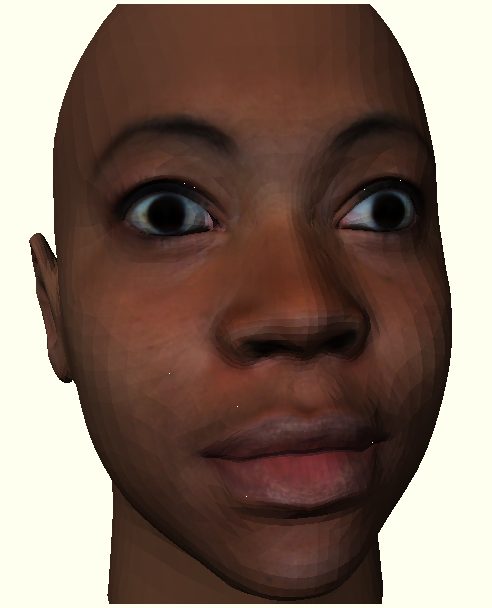
\includegraphics[width=0.7\textwidth]{holes-in-model.png}
\caption{Отверстия в модели при тесселляции}
\label{fig:holes-in-model}
\end{figure}

Тесселляция - прием, с помощью которого можно увеличить количество
многоугольников в полигональной трёхмерной модели. В процессе тесселляции
объектов, составленных целиком из треугольных полигонов \footnote{В случае
использования четырехугольных полигонов добавление новых вершин необязательно,
достаточно поделить диагональю каждый полигон пополам}, необходимо добавлять
новые вершины. В этом крылась первая проблема: объекты движка ``Three.js'',
загруженные в буферы WebGL, не могут изменить количество вершин, содержащихся в
их геометрии. Так как объект загружается в буферы WebGL при первом отображении
сцены, то для обхода этой проблемы нужно было либо тесселлировать объекты только
один раз до необходимого размера ребра непосредственно после загрузкой и до
отображения сцены, либо динамически тесселлировать объект, удалять его со сцены
и пересоздавать. Преимущество первого метода над вторым в том, что он не
затрагивает производительность приложения и несомненно является более простым в
реализации, однако он не позволяет добиться динамической тесселляции, которая
становится доступной при использовании второго метода. При разработке
планировалось опробовать алгоритм тесселляции с использованием первого метода, а
потом перейти на динамическую тесселляцию при достижении хороших результатов на
первом этапе.

В качестве реализации алгоритма тесселляции была взята версия алгоритма,
входящего в стандартную поставку фреймворка ``Three.js''. Однако при предварительном
тесселлировании объектов и их дальнейшем отображении была
выявлена серия проблем.

\begin{itemize}
    \item При тесселлировании простейших геометрических фигур с четырехугольными
    гранями сбиваются цвета граней
    \item При тесселлировании загруженных *.OBJ-объектов в модели появляются
    отверстия в местах стыках граней
\end{itemize}

Если четырехугольные грани являются довольно редким объектов при задании
геометрии объектов, то второй недостаток существенен при работе с моделями.
Самостоятельное изучение кода тесселляции никаких результатов в
исправлении недостатка алгоритма не дало. Отчет об ошибке вместе с примерами
кода был отправлен разработчикам, а изменения в коде приложения,
связанные с тесселляцией, были вынужденно откачены назад.

